\chapter{Preparation}

\section{Theory}
% Commonly two kinds of photodetectors are used. PIN-Photodiodes and Avalanche Photo Diodes (APD).
\subsection{PIN-Photodiode}


\begin{figure}%
\centering
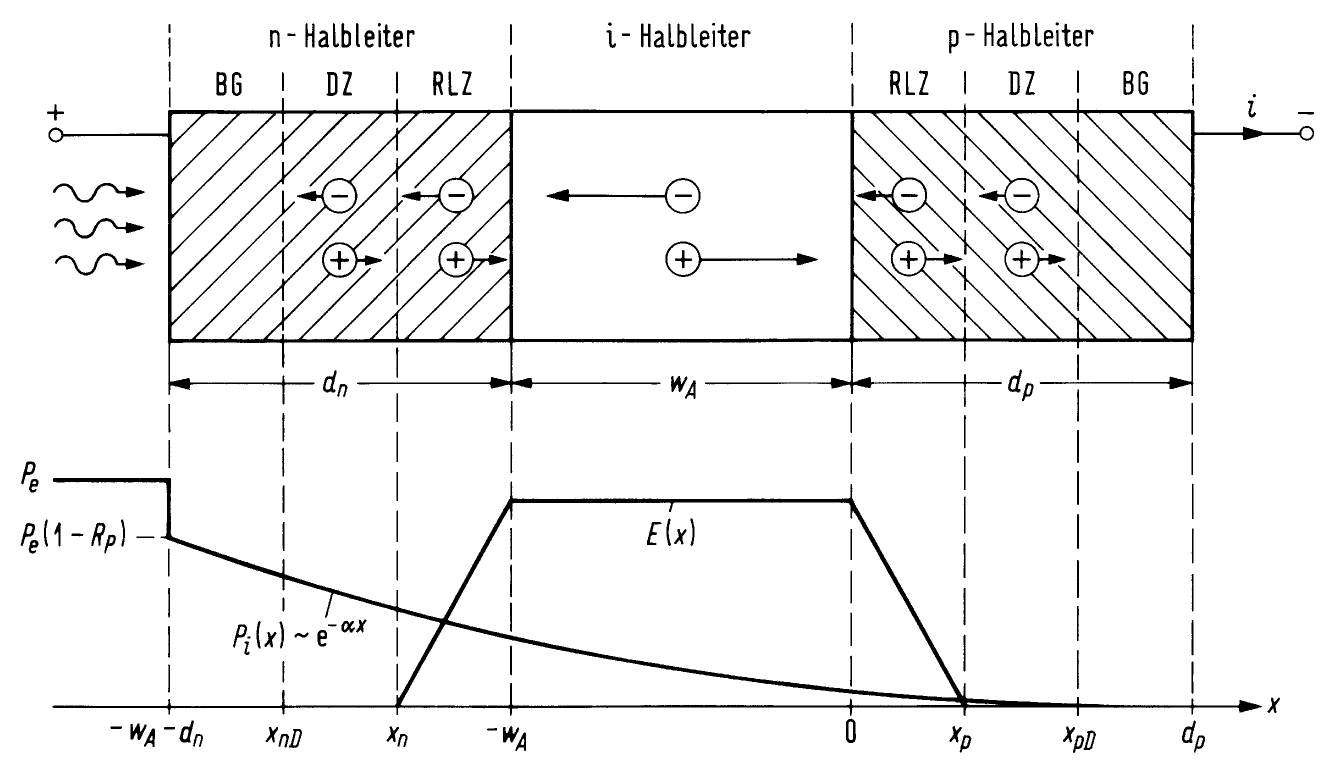
\includegraphics[width=.5\columnwidth]{Grafiken/pin.png}%
\caption{Layout of a PIN-diode}%
\label{fig:pin}%
\end{figure}


\begin{figure}%
\centering
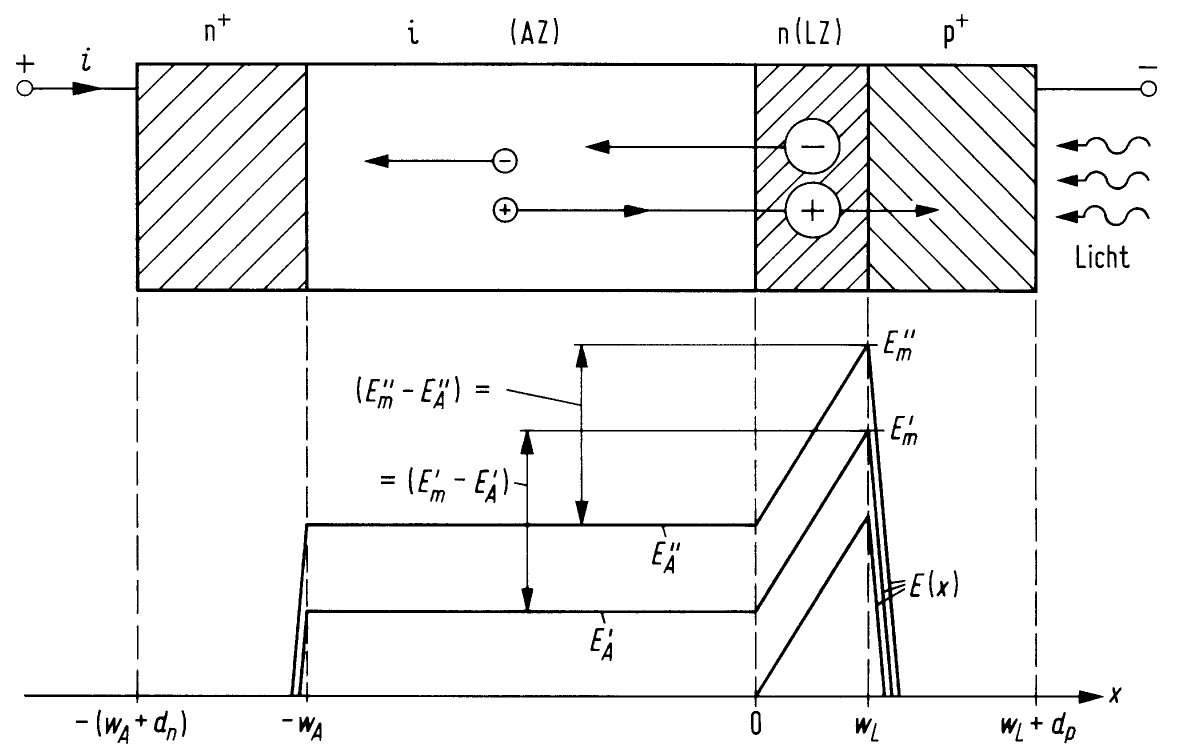
\includegraphics[width=.5\columnwidth]{Grafiken/apd.png}%
\caption{Layout of an APD}%
\label{fig:APD}%
\end{figure}

In a PIN-Photodiode a p-doped region of a semiconductor is seperated from a n-doped region by an intrinsic zone. This layout is shown in figure \ref{fig:pin}. If the device is irradiated, photons with more energy than the band gap ($h\cdot f > W_{\mathrm{Gap}}$) are absorbed by generating a electron hole pair. Usualy this electron hole pair recombines after a short period of time, but if it is generated in the space charge zone or the intrinsic zone of a pin junction the charge carriers are accelerated by the electric field in opposite directions. This carrier movement in the device is compensated by a current in the external wiring.

A electron hole pair generated in the diffusion zone also leads to a current. Since the carriers in that zone move with their diffusion velocity, which is orders of magnitude smaller than the drift velocity in the intrinsic zone, generation in the diffusion zone is not wanted. The generation of carriers in the diffusion zone can be minimized by highly doping the semiconductor.\footnote[1]{Optische Nachrichtentechnik; Grau,G; Freude, W; 3rd ed. Springer, 1991}


\subsection{Avalanche Photo Diode (APD)}
% The setup of a APD is shown in figure \ref{fig:APD}. It is build like a PIN-diode, but there is an additional avalanche zone. 
The APD is build similary to the PIN-diode. There is a n-doped zone at the one side and a p-doped zone at the other side. In between there is also a intrinsic domain and additionaly another doped zone, which is oppositly doped as the contigous zone (cf. figure \ref{fig:APD}. Like in the PIN-diode, the carriers are generated in the i-zone and accelerated in different directions. One kind of the carriers (in the figure \ref{fig:APD} the holes) move through the avalanche zone. There carriers are accelerated by the high electric field. These carriers have enough kinetic energy to generate further carriers by impact ionization. This leads to a amplification of the current induced by one photon. Since the carrier multiplication in the avalanche zone is a stochastic process, there is more noise in the APD than in the PIN-diode.\footnotemark[1]

\subsection{Other stuff}
\todo{Kapitelname �ndern!!!!!!!!!!!!}

The photo current $i$ of photo diode is proportional to $S\cdot P_{\mathrm{e}}$ with the optical power $P_{\mathrm{e}}$ and the sensitivity $S$ of the photo diode.

The sensitivity is given by

\begin{equation}
S = \frac{\eta e \lambda_{\mathrm{L}}}{hc}
\label{eq:}
\end{equation} 
where $h$ is Planck's constant, $e$ the elementary charge, $\eta$ the quantum efficiency and $\lambda$ the wavelength of the incoming light. 
Since $\eta$ depends strongly on the absorption $\alpha$. The absorption depends on the wave length. For $\lambda > \lambda (W_{\mathrm{gap}})$ nothing gets absorbed by the material and $\eta = 0$. For $\lambda < \lambda (W_{\mathrm{gap}})$ the sensitivity gets worse es well. The energy of the photons are higher than the band gap energy. This additional energy changes into phonon energy.\footnote[2]{Optical Communication Systems - Part 2, Wolfgang Freude}

Figure \ref{fig:sens} shows the spectral sensitivity of a BPW34 PIN photodiode\footnote[4]{Vishay Semiconductors, BPW34 Datasheet}. 

\begin{figure}%
\centering
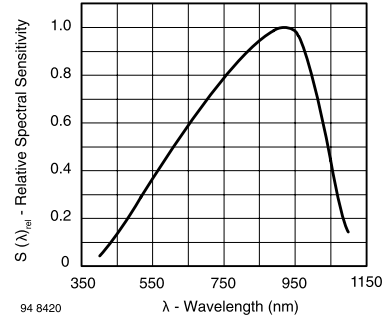
\includegraphics[width=.4\columnwidth]{Grafiken/sensitivity.png}%
\caption{Relative Spectral Sensitivity vs. Wavelength.$^4$}%
\label{fig:sens}%
\end{figure}



\section{Question 1: Open Circuit Voltage}
The Term (1)
\begin{equation}
 I_{\mathrm{PIN}} = I_{\mathrm{Sat}}\left[\exp\left(\frac{U_{\mathrm{PIN}}}{U_{\mathrm{T}}}\right)-1\right] -I_{\mathrm{pr}}
\label{eq:diode}
\end{equation}
from the experiment description, with $R_{\mathrm{a}}\to\infty(I_{\mathrm{PIN}}\to0)$ can be rearranged to:
\begin{equation}
 I_{\mathrm{pr}} = I_{\mathrm{Sat}}\left[\exp\left(\frac{U_{\mathrm{PIN0}}}{U_{\mathrm{T}}}\right)-1\right]
\end{equation}
and further to:
\begin{equation}
 U_{\mathrm{PIN0}}(I_{\mathrm{pr}}) = U_{\mathrm{T}}\ln\left(\frac{I_{\mathrm{pr}}}{I_{\mathrm{Sat}}}+1\right)
\end{equation}

\section{Question 2: Electrical Power of a PIN Diode}

With $P = R\cdot I^2$, $I_{\mathrm{pr}} = S\cdot P$ and equation \eqref{eq:diode}, the Power of the PIN-diode can be calculated by:
\begin{equation}
 P_{\mathrm{el}} = R_{\mathrm{a}}\cdot\left\{ I_{\mathrm{Sat}}\left[\exp\left(\frac{U_{\mathrm{PIN}}}{U_{\mathrm{T}}}\right)-1\right] -S\cdot P\right\}^2.
\label{eq:power}
\end{equation}
For the Case:
\begin{equation}
 \frac{U_{\mathrm{PIN}}}{U_{\mathrm{T}}} \ll 1 \to \exp\left(\frac{U_{\mathrm{PIN}}}{U_{\mathrm{T}}}\right)\approx1+\frac{U_{\mathrm{PIN}}}{U_{\mathrm{T}}}
\label{eq:vereinfachung}
\end{equation}
equation \eqref{eq:diode} can be simplified to:
%\begin{equation}
%  P_{\mathrm{el}} = R_{\mathrm{a}}\cdot\left\{ I_{\mathrm{Sat}}\cdot\frac{U_{\mathrm{PIN}}}{U_{\mathrm{T}}} -S\cdot P\right\}^2.
%\end{equation}
%
%Because of \eqref{eq:vereinfachung} the primary photo current $S\cdot P$ is dominating. 
\begin{equation}
I_{\mathrm{PIN}} = I_{\mathrm{Sat}}\cdot\frac{U_{\mathrm{PIN}}}{U_{\mathrm{T}}} -S\cdot P
\label{eq:}
\end{equation}
The power $P = U_{\mathrm{PIN}} \cdot I_{\mathrm{PIN}}$ can be maximized  by deriving $P$ by $U_{\mathrm{PIN}}$. That way the voltage for the maximum power can be obtained. 
\begin{equation}
U_{\mathrm{PIN}} = \frac{S\cdot P \cdot U_{\mathrm{T}}}{2\cdot I_{\mathrm{sat}}} 
\label{eq:}
\end{equation}
Inserting this therm into \eqref{eq:diode} the current for the maximum power is

\begin{equation}
I_{\mathrm{PIN}} = - \frac{S \cdot P}{2}
\label{eq:}
\end{equation}

Thus for $R = U/I$ the resistance for the maximum power is

\begin{equation}
R_{\mathrm{max}} = - \frac{U_{\mathrm{T}}}{I_{\mathrm{Sat}}}
\label{eq:}
\end{equation}

For the maximum power then results:
\begin{equation}
 P_{\mathrm{max}}= \frac{S^2\cdot P^2\cdot U_{\mathrm{T}}}{4 \cdot I_{\mathrm{sat}}}
\end{equation}

%\todo{da stimmt irgendwas noch net}

\section{Question 3: Photodetector with Transimpedance Amplifier}

\begin{figure}[h]%
\centering
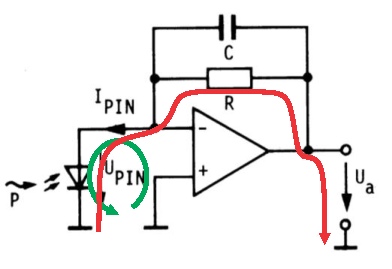
\includegraphics[width=.8\columnwidth]{Grafiken/OPAMP_m.pdf}
\caption{}%
\label{fig:OPAMP}%

\end{figure}

In Figure \ref{fig:OPAMP} with Kirchhoff's second law it can be derived (using the red loop):
\begin{equation}
 - u_{\mathrm{PIN}} - i_{\mathrm{PIN}}\cdot \frac{R}{1+ j\omega RC}+u_{\mathrm{a}} = 0 .
\label{eq:masche1}
\end{equation}
Using
\begin{equation}
 u_{\mathrm{PIN}}=0.
\label{eq:masche2}
\end{equation}
resulting also from Kirchhoff's second law (green loop) you get:
\begin{equation}
 u_{\mathrm{a}} = i_{\mathrm{PIN}}\cdot \frac{R}{1+ j\omega RC}.
\label{eq:ua}
\end{equation}

For the cut-off frequency $f_{\mathrm{3dB}}$ the following condition has to be fulfilled:
\begin{equation}
 \left|\frac{u(f_{\mathrm{3dB}})}{u(0)}\right| = \frac{1}{\sqrt{2}}
\end{equation}
With \eqref{eq:ua} you obtain
\begin{equation}
 \left|\frac{i_{\mathrm{PIN}}\cdot \frac{R}{1+ j2\pi f_{\mathrm{3dB}} RC}}{i_{\mathrm{PIN}}\cdot R}\right| = \frac{1}{\sqrt{2}}
\end{equation}
and further
\begin{equation}
 f_{\mathrm{3dB}} = \frac{\sqrt{2}-1}{2\pi RC} 
\end{equation}

With \eqref{eq:ua}, \eqref{eq:diode},\eqref{eq:masche2} and $I_{\mathrm{pr}}=S\cdot P$ it can be obtained:

\begin{equation}
 u_{\mathrm{a}} =  -S\cdot P\cdot \frac{R}{1+ j\omega RC}
\end{equation}

Because in a stationary case $i$ is proportional to eFg it is also proportional to $P_e$. Here $e$ is the elementary charge, $F$ the active surface and $g$ the optical generation rate.
 
The multiplication in the APD is caused by impact ionization. The ionization probabilities $\beta_i$ and $\alpha_i$ are proportional to $e^{\frac{-W_{\mathrm{ion}}}{W_T}},  W_T=eEl_\mathrm{LO}$. Here $E$ is the electrical field, $l_\mathrm{LO}$ the free path. Therefore $\beta_i$ and $\alpha_i$ are independent of $P$.


Thus for a constant $\omega$, $u_{\mathrm{a}}$ is linearly dependent on the optical power $P$. The proportionality constant is 
\begin{equation}
\zeta = -S\cdot \frac{R}{1+ j\omega RC}.
\label{eq:}
\end{equation}
\comseb{Hier steht noch rot "Betr�ge!" am rand. die beiden letzten formeln k�nnen aber ja eigentl schon complex sein. Bei der 2. kann ma sichs h�chstens nochma �berlegen.}
\section{Question 4: APD - Change of light power}

%\begin{equation}
%eFg_{\mathrm{photo}} = \frac{\eta e}{hf_L}P_e\frac{\alpha e^{-\alpha(x+w_a)}}{1-e^{-\alpha w_A}}, \rightarrow eFg_{\mathrm{photo}} \propto P_e.
%\label{eq:}
%\end{equation}
%
%Because in a stationary case $i$ is proportional to eFg it is also proportional to $P_e$. Here $e$ is the elementary charge, $F$ the active surface and $g$ the optical generation rate.
% 
%The multiplication in the APD is caused by impact ionization. The ionization probabilities $\beta_i$ and $\alpha_i$ are proportional to 
%\begin{equation}
%\alpha_i, \beta_i \propto e^{\frac{-W_{\mathrm{ion}}}{W_T}},  W_T=eEl_\mathrm{LO}.
%\label{eq:}
%\end{equation}
%
%
%Here $E$ is the electrical field, $l_\mathrm{LO}$ the free path. Therefore $\beta_i$ and $\alpha_i$ are independent of $P$.
%
%Since $M_0$ is for the stationary case (dP/dt=0)
%\begin{equation}
%M_0=\frac{(\beta_i  -\alpha_i)e^{(\beta_i-\alpha_i)w_L}}{\beta_i - \alpha_i e^{(\beta_i - \alpha_i)w_L}},
%\label{eq:}
%\end{equation}
%$w_L$ is the length of the avalanche-zone, $M_0$ does not depend on $P$.
%with the differential equation
%
%\begin{equation}
%\frac{1}{v_p} \frac{\partial i_p}{\partial t} +\frac{\partial i_p}{\partial x} = eFg_{\mathrm{photo}} 
%\label{eq:}
%\end{equation}
%
%and
%
%\begin{equation}
%\frac{1}{v_n} \frac{\partial i_n}{\partial t} +\frac{\partial i_n}{\partial x} = eFg_{\mathrm{photo}} 
%\label{eq:}
%\end{equation}
%
%follows for $\frac{\partial}{\partial t} = 0$
%
%
%\begin{equation}
%i_p = eFg_{\mathrm{photo}}\cdot x
%\label{eq:}
%\end{equation}
%
%\begin{equation}
%i_n = eFg_{\mathrm{photo}}\cdot x
%\label{eq:}
%\end{equation}
%
%Therefore $i_n$, $i_p$ $\propto P_e$.
%
%At a APD there's an impact ionszation. 
%\begin{equation}
%eFg_{\mathrm{ion}} = \alpha_i i_n + \beta_i i_p
%\label{eq:}
%\end{equation}

The in figure \ref{fig:Q4_APD}\footnote[3]{Source: OKT Experiment 2: Photodiode analysis task-sheet} shown circuit is given.
The APD gets radiated by a power $P$. 
When changing the radiating power to $P + \Delta P$ several things change in the circuit.

The circuit is driven by a constant voltage of $U = 0.9\cdot U_{\mathrm{BR}}$. When changing $P$, $I_{\mathrm{APD}}$ changes proportional to the change of $P$.

A change of $I_{\mathrm{APD}}$ causes a change of the voltage that falls off over $R_{\mathrm{V}}$. Since the driving voltage is constant, the voltage over the APD decreases. Because $M_0$ depends strongly on $U_{\mathrm{APD}}$, $M_0$ decreases as well. 





\begin{figure}%
\centering
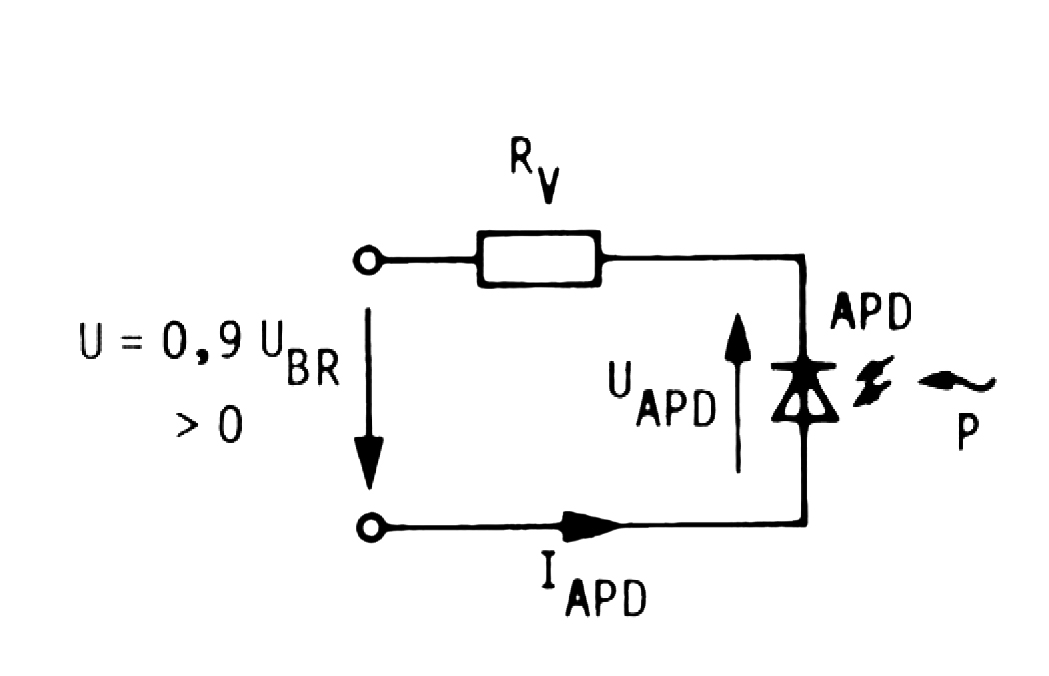
\includegraphics[width=.5\columnwidth]{Grafiken/Q4_APD.jpg}%
\caption{APD with series resistance}%
\label{fig:Q4_APD}%
\end{figure}


